% 115 120
\documentclass[12pt,a4paper]{amsart}
\usepackage[slovene]{babel}
\usepackage[utf8]{inputenc}
\usepackage{amsmath,amssymb,amsfonts}
\usepackage{url}
\usepackage[dvipsnames,usenames]{color}
\usepackage{graphicx} 


\begin{document}
\title{Grafitti Conjecturre 194}
\author{Martin Praček, Mela Malej}
\maketitle
Za predmet Finančni praktikum v študijskem letu $2018/19$ Martin Praček in Mela Malej dobila nalogo predstaviti problem Grafittijeve konjekuture $194$. \\\\
\section{Predstavitev problema}
Grafittijeva konjektura 194 nam zastavi vprašanje iz teorije grafov.Zanima nas, ali za vsak preprost, povezan graf, ki zadošča pogoju $$ \alpha(G) \leq 1 + \lambda_{avg}(G)$$, velja, da obstaja hamiltonska pot. Gre za računalniško generirano trditev, pri kateri nas zanima, ali lahko najdemo protiprimer.\\
\section{Pogoji našega problema}
Naš pogoj je torej $$ \alpha(G) \leq 1 + \lambda_{avg}(G),$$
kjer je $G$ naš graf, $\alpha(G)$ je neodvistnostno število, $\lambda_{avg}$ pa je povprečna lokalna neodvistnost grafa.\\
\ \\
\textbf{Neodvistnostno število grafa} $\alpha(G)$ nam pove moč največje množice, ki vsebuje  vozlišča grafa $G$, od katerih nobeni dve niste sosednji.\\
\ \\
\textbf{Lokalna neodvistnost grafa} $\lambda(G, v)$ nam pove neodvistnostno število podgrafa $Gv$ grafa $G$, kjer je $Gv$ definiran na sosedih vozlišča $v$. $\lambda_{avg}(G)$ nam pove povprečno lokalno neodvistnost.\\
\begin{figure}[h]
	\centering
	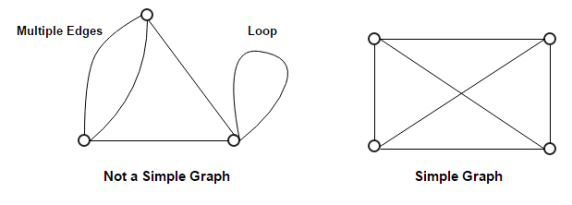
\includegraphics[scale=1]{slike/graf1}
\end{figure}

Ves čas zahtevamo, da je graf \textbf{preprost in povezan}. Ta zahteva pomeni, da ne obstaja vozlišče, ki ne bi bilo sosednje vsaj enemu drugemu vozlišču, poleg tega pa med dvema povezavama obstaja kvečjemu ena povezava in ne obstaja  povezave od vozlišča $v$ do vozlišča $v$, kar pomeni da ne obstajajo zanke na enem vozlišču.\\
 
Graf ima \textbf{hamiltonsko pot}, če obstajata dve vozlišči, ki ju povezuje pot, ki natančno enkrat obišče vsako vozlišče grafa.\\
\ \\
Najina naloga je torej na dovolj velikem vzorcu grafov pokazati da to velja, ali pa dobiti protiprimer, ki bo dokazal da to ne drži.\\
\section{Dosedanje delo}
Do sedaj sva začela s pisanjem kode, ki bo preverjala majhne grafe, torej do približno $30$ vozlišč. Za tako ločnico sva se odločila zaradi nekaj NP-težkih problemov, s katerimi morava v najini seminarski nalogi delati. Pri tem izstopata predvsem problem Hamiltonske poti, ter določitev neodvistnostega števila grafa. \\
Problem neodvistnostnega števila grafa za male grafe sva rešila z zaenkrat še nedelujočo kodo v datotekah \begin{verbatim}dodatna_pomoc_mali_grafi.py\end{verbatim} ter \begin{verbatim}mali_grafi_neenakost.py\end{verbatim}. Tu sva uporabila iterativni postopek, kjer sva določila potenčno množico vseh možnih naborov vozlišč grafa, in nato ugotovila velikost največje množice, katere elementi med seboj niso sosedi.\\
Še večji problem predstavlja problem Hamiltonske poti, ki sva jo delno rešila za male grafe v \begin{verbatim}mali_grafi_hamilton.py\end{verbatim}, vendar najine kode še nisva dokončala.  \\

Delo, ki sva ga do sedaj naredila, temelji predvsem na algoritmih za manjše grafe. Najin program se bo izvedel v \begin{verbatim}
izvaja_mali_grafi.py
\end{verbatim}, ki bo v vseboval zgolj eno funkcijo z eno for zanko, ki bo šla skozi vsa števila od 0 do 30 in zanje izvedla sledeč postopek.\\
Najprej nam bo generator, ki še ni dokončan vrnil vse grafe, ki bodo velikosti, kolikor bo v tistem trenutku vrednost for zanke.\\
 Nato bodo ti grafi šli skozi dodatna testiranja, da bomo preverili, ali zadoščajo pogojem, določenim s definicijo problema. Najprej bo preverjeno, če je graf povezan. Sledilo bo preverjanje enostavnosti grafa. Na ta način bova število grafov, ki jih bova morala testirati, precej zmanjšala. \\
 Nato bova za grafe, ki bodo preostali, določila neodvistnostno število $\alpha$ ter lokalno neodvistnostno število $\lambda_{avg}$. Ko bo to določeno, bova izbrala le tiste grafe, ki bodo zadoščali naši neenakosti. \\
 Za grafe, ki bodo prestali vse izbore bo potem sledil še zadnji test; testirala bova, ali obstaja hamiltonska pot. Če nama uspe najti protiprimer, bova te protiprimere shranila posebej.
\section{Prihodnje delo}
Najino nadaljne delo bo predvsem delo na velikih grafih. Zato se bova morala poglobiti tudi v metahevristiko, ki pa se ji do sedaj nisva še veliko posvečala. Zavedava se, da bova morala najino kodo precej spremeniti, saj najine rešitve NP-težkih problemov niso narejene za delovanje v polinomskem času.
\end{document}